\PassOptionsToPackage{bookmarks=false}{hyperref}
%% The first command in your LaTeX source must be the \documentclass command.
%\documentclass[sigconf]{acmart}
\documentclass[sigconf]{acmart}
\usepackage{xspace}
\usepackage{hyperref}
\usepackage{listings}
% \usepackage[ruled,vlined]{algorithm2e}
\usepackage{overpic}
\usepackage{amsmath}
\usepackage{alg}
\usepackage{subcaption}

\lstset{language=Java, showspaces=false, showtabs=false, breaklines=true,
  numbers=left, numbersep=1pt, numberstyle=\tiny\color{black},
  showstringspaces=false, breakatwhitespace=true, commentstyle=\color{pgreen},
  keywordstyle=\color{pblue}, stringstyle=\color{pred},
  basicstyle=\small\ttfamily, moredelim=[il][\textcolor{pgrey}]{$$},
  moredelim=[is][\textcolor{pgrey}]{\%\%}{\%\%}}

\newcommand{\name}{NAME\xspace}
\newcommand{\fixme}[1]{{\color{red}{\textbf{FIXME:#1}}}}

\AtBeginDocument{%
  \providecommand\BibTeX{{%
    \normalfont B\kern-0.5em{\scshape i\kern-0.25em b}\kern-0.8em\TeX}}}

\begin{document}

\title{Critical Survey 2: Relational Parametricity}

\author{Juyeon Yoon}
\affiliation{%
  \institution{School of Computing, KAIST}
  \country{greenmon@kaist.ac.kr}\\\vspace{2em}
}


\maketitle

\section{Introduction}
\label{sec:intro}

When we use strictly-typed programming languages, we necessarily eager the existence of some \textit{general} type to reduce the duplicated code lines that hurt our fingers. In other word, it is quite likely to process program elements in a similar way, although those are in different types. In fact, there already are - such as a Generic type in Java, template in C++. In this paper, we dive into the theoretical basis on those convenient features for supporting \textit{polymorphsm} with parametricity. 

Before discussing relational parametricity directly, we cover the exact meaning of polymorphism, and its categories. As a (non-interesting) spoiler, the specific category of parametric polymorphism becomes a key actor supported by sound formalisation of `relation' view of types. 

\section{Polymorphism}

The notion of \textbf{polymorphism} was introduced earlier (in 1960s), by providing a single interface for multiple-typed program entities. 

There are several classes of polymorphisms, such as:
\begin{itemize}
  \item Ad hoc polymorphism
  \item Parametric polymorphism
  \item Inclusion polymorphism (subtyping)
\end{itemize}

% explain inclusion polymorphism?

In a more historical context, the term first introduced by Christopher Strachey with an important classification: ad hoc polymorphic functions and parametric polymorphic function. Overloading, allowing to use the same name of the functions with different types, is the typical example of ad hoc polymorphism. Meanwhile, parametric polymorphism provides convenient, but theoretically more complex features for handling polymorphic behavior of functions. One needs to write a definition of a function once, but treat the argument (return) types as variables, which can be instantiated at many possible concrete types. Starting from the first language \texttt{ML} implementing parametric polymorphism, may programming languages like \texttt{OCaml}, \texttt{F\#}, \texttt{Haskell} supports it as language features, and \texttt{Java}, \texttt{C\#} introduced \texttt{generics} for it. The paradigm of generic programming has got also popular with its powerful ability for abstracting useful algorithms to cover more diverse data structures. 

`template' supported in \texttt{C++} is a little bit different. Superficially it is the same with other languages in the way of supporting paramteric polymorphism, with just looking at the resulting behavior, but in compile time the separate functions are generated with concrete types. Hence, the final compiled implementation executes the different function with given type, with no general entry point, of which internal behavior in fact is more close to ad-hoc polymorphism.

\subsection{Difference between Ad-hoc Polymorphism and Parametric Polymorphism}

% further discuss in what sense parametric polymorphism differs from ad-hoc polymorphism.
Except for overloading, there is one more example of ad-hoc polymorphism, which is coertion. Coertion is a type conversion to match the provided argument type with the parameter type required from the function definition. There are language rules defining the conversions among primitive types, using the type constructor and conversion operators.

The general idea on ad-hoc polymorphism is, it just focuses on the \textit{apparent} perspective of polymorphism, not guaranting the universal behavior among the actual invocation of the function with different types. On the other hand, parametric polymorphism uses a single definition of function, or method, hence the behavior is intrinsically uniform for all types applied. Hence, we can say that parametric polymorphism guarantees not only genericity~(apparently compatible different types), but also parametricity~(the uniform behavior for any type of arguments).

\subsubsection{Parametric Polymorphism on Data Types}

The concept also applies for data types, additional to functions. For example, list, or array that can contain arbitrary types can be regarded as polymorphic data type.

% Parametric polymorphism to enhance 'expressiveness' of programming language
% wait, type polymorphism is different from parametric polymorphism?

\subsection{Subtyping}

There remaining one category of polymorphism is inclusion polymorphism (subtyping). Providing substitutability, any method or functions implemented on supertype can also operate on elements of the subtype. (this notion looks similar to Liskov substitution rule in OOP principles) Personally, I was more familiar with the interpretation of polymorphism in this context, because the term is commonly used in object-oriented programming (for parametric polymorphism, generic programming is the corresponding paradigm). The user-defined type is regarded as interface in OOP languages, and the subtyping is implemented as interface inheritance in those languages.

Combining parametric polymorphism with subtyping should provide the most convenient way for supporting polymorphsms, many function programming languages support both features, still some theoretical perspectives remain to be researched.


\section{Relational Parametricity}
\label{sec:relparam}

From the classic paper~\cite{ParametricPolymorphism} written by Reynolds, the way of formalising parametric polymorphism is discussed. Because the previous attempts on algebraically formalising polymorphic type system relying on homomorphism on function failed to account for higher-order functions, he introduces the generalization of using relation instead of function. As a result, he found that types could be view abstraction that enables representation independence, information hiding, naturality or parametricity.~\cite{2013dedicate} As an extension of typed lambda calculus, Reynolds and Girard co-developed polymorphic lambda calculus, sometimes called by the cool name, \texttt{System F}. 

\subsection{Abstraction Theorem (Parametricity Theorem)}

Here, the important finding of Abstraction Theorem (later becomes the basis for justifying the notion of parametricity) is introduced. Abstraction Theorem is briefly about connecting the meaning of expressions under different (specifically, differently-typed) related arguments. Hence, to interpret the meaning of polymorphic function, we don't need to `look inside' what the actual parameter type is. The sort of universality is guaranteed by this theorem, in a sentence, \textit{do the same thing, not caring about what the types are!}

Reynolds denotes that the initial attempt for using set for representing each type was failed, by demonstrating that the traditional set-theoretic model does not fit to the polymorphic lambda calculus. The earlier paper from Reynolds contains proof that there is no set-theoretic models which preserve the function space and binary product and satisfy some weak condition on universal quantification~\cite{nosettheoretic}, causing that an attempt of formalising a polymorphic type to unintentially allow some functions that don't do the same computation on some types. 

\subsection{Relation instead of Set}

To explain why the set-theoretic view of parametric polymorphism doesn't hold, a representative example borrowed from a \textit{StackExchange} post (\url{https://cstheory.stackexchange.com/questions/19548/how-can-relational-parametricity-be-motivated}) is presented:

\[\forall X : \texttt{Type.}\, X \rightarrow X \]

With set-theoretic semantics, the original intention of identity map doesn't preserved with the below exceptional case with different meaning:

\[\lambda X : \texttt{Type.}\, \lambda a : X.\: \texttt{if} \left( X = \{0, 1\} \right) \texttt{then} \: 0 \: \texttt{else} \: a \]

To avoid this situation, relational semantics could be used instead of set semantics. 


Although the other paper by Andrew Pitts, showed that some constructive theories enable polymorphisms to preserve the intended interpretations for the function spaces and products, but I think that in the perspective of viewing logical relations as generalised many-to-many correspondence (I borrowed the interpretation from the other reply in the above \texttt{StackExchange} post which helped me to get intuition about it) from the one-to-one isomorphism, and many-to-one homomorphism previously explained with algebraic view, I think the relational semantics would have value on the capability of more expressively describing polymorphic-typed languages.


\subsubsection{Identity Relation}

To give a relational equivalent for constant types such as \texttt{Bool} and \texttt{Int}, identity relations are used. 

\subsubsection{Type Constructor}
for each type constructors, (cartesian product, disjoint union, implication, quantifiers) the constructed types get to be a relation according to the corresponding components' relations. 


\subsection{Polymorphic-typed Lambda Calculus}

As explained in the paper~\cite{PolymorphicLambdaCal}, to support the definition of polymorphic types based on the relational model explained above, the traditional typed lambda calculus is extended by treating types as variables. A surprising consequence is that every expression of the polymorphic typed lambda calculus reduced to $\beta$-normal form, which guarantees termination of the expression. However, it also means that the expressiveness of this language restricts to terminating expressions only, missing some useful infinite data structures in practice. Moreover, polymorphic function encodes a proof by treating type constructors(such as $\rightarrow, \times, + $) as logical connectives. This fact seems to be somewhat related to the parametricity theorem. From the example in the paper, the premitive types such as boolean and natural numbers can be also encoded as polymorphic types. For example,

\[ \textbf{bool} = \triangle t. \: t \rightarrow \left( t \rightarrow t \right) \]

which also correctly encodes the meaning of boolean as binary choice function. Although not be certain, with my intuition, the theorems derived from these expressive types would provide more abundant information that explains the behavior of the function.  

So the question remains, \textit{how does the relational model interpret polymorphic-typed lambda calculus to produce appropriate semantics?} The type environment for mapping type variables into the relation, that interprets each type as a relation. To successfully support parametricity in the semantics, note that we choose relational model instead of the naive set-theoretic model having the issue explained above.


\subsection{From Representation to Application}

Parametricity Theorem introduced from the paper~\cite{theoremsforfree}, which can be seen as an important variant of Abstraction Theorem, focuses on constructing general meaning of (polymorphic) data structures, (polymorphic) functions regardless of the concrete types, only relying on the relation of components, for example, elements, arguments, types, results. In other words, parametricity theorem provides specific applications by deriving `useful' properties, or theorems only looking at the ingrediant types (in case of type variables such as \texttt{List<T>}), or types of the arguments (in case of functions such as \texttt{F: T $\rightarrow$ T}). That's why the title of paper is \textit{$<$Theorems for free!$>$}, and in my opinion, the change of the view from the universal representation of the different types, or different-typed functions in Abstraction Theorem to the universal \textit{meaning} of the polymorphic type or function based on their abstract types is important because the from the derived theorem we can capture the general pattern among same types; author mentions some immediate `useful' application of the theorems such as algebraic manipulation, derivation of an algorithm for compiling pattern matching in functional languages, and VLSI circuits. Although it was a little bit hard to imagine the concrete procedure of those application mentioned, for designing some higher-order functionalities, the derived theorems for the argument type should explain the actual meaning of the argument not necessarily looking at the actual implementation. As mentioned in the paper, the more specific the type system is, the more expressive provided information from the theorems derived from the type will be. There is also an interesting view of considering parametricity as a dual to abstraction: "where abstraction hides details about an implementation from the outside world, parametricity hides details about the outside world from an implementation."~\cite{parametricitylecture}


\subsection{Categorical View}
As covered in the lecture, adopting the view of Category Theory, type constructors can be view as functor, and the parametric polymorphic functions can be regarded as natural transformation. The logical relations for expressing types with polymorphism corresponds to morphism in Category Theory. Natural transformation that maps with functors, again, can be interpreted as applying the same behavior for all types (which corresponds to Objects) by preserving the morphisms (corresponds to logical relations). Following commutative diagram borrowed from the paper~\cite{2013dedicate} shows the correspondence more clearly. ($\eta$ denotes natural transformation, and F, G are functors.)

\begin{figure}[!h]
  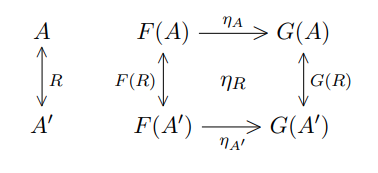
\includegraphics[width=150px]{images/commute.png}
\end{figure}

\subsection{Relational Parametricity vs. Interface Inheritance}
The concept of relational parametricity reminded me somewhat similar property of \textit{Duck Typing} in Object-Oriented Programming. They are similar in the common goal of desiring the popular, and important strategy of abstraction in computer science. However, unlike focusing on abstracting the implementation of the inclusion parametricity, I think that relational parametricity is more about generalizing relations among arguments and results, so help the developer to produce more universal implementation by capturing the general pattern which can be treated equivantely for variety of types: facilitating \textit{cleaning} rather than \textit{hiding}.



\section{Recent Research}
\label{sec:recent}


\subsection{Type Inference}
For the explicitly typed form of lambda calculus, type inference is trivial. However, the explicit effort for annotating types whenever a variable is bound should be a significant burden to a programmer, practically we need an algorithm to decide the types on an untyped lambda calculus. It has been proved that the complete type inference in System F (without explicit type annotations) is impossible. With some restriciton on the language feature allows a type inference algorithm, but recent tendency is alleviating restrictions and using more expressive type system, such as GADT (Generalized Algebraic Data Type) in OCaml. 

\subsection{Combining Subtyping with Parametric Polymorphism}
There exists a slightly later work introducing an extension of System F, called F-sub, that combines parametric polymorphism with subtyping record. This direction could make functional programming languages also enjoy the fruitful features in object-oriented languages that construct type hierarchy.

\subsection{Heap Parametricity}
Applying the relational semantic model for treating the point-addressed shared mutable data structures even combined with polymorphic behavior is a fresh research direction. There is a professor Yang's previous work~\cite{yang08} applies relational parametricity on the higher-order data strutures on heap, discovering a way of applying a parametric model for separation logic with the idea of defining semantics in continuation-passing style. The success in defining the parametric model of separation logic is notable, but there seems to be remaining broad research opportunity on reasoning the complex data structures using the parametric model. What if the each element of compositional data structure on heap has the polymorphic type? How about the list can contain elements of generic types? I also wonder whether it is possible to express the polymorphic functions accepting pointer variable as an argument in a formal way.

\section{Conclusion}
\label{sec:conclusion}

We discussed general notion of polymorphism, especially on the parametric polymorphism with the paradigm of generic programming, intuitions in terms of abstraction, and the categorical view for interpreting parametricity. Due to the lack of experience on functional programming, the explanation on formalisation of relational parametricity in this paper might contain some error. However, understanding the functional-language style polymorphism and the theoretical basis behind the popular functional languages was very valuable experience to me (the author of this critical survey).

\bibliographystyle{ACM-Reference-Format}
\bibliography{newref}

\end{document}

